

\documentclass{article}

% Language setting
% Replace `english' with e.g. `spanish' to change the document language
\usepackage[english]{babel}
\usepackage{xeCJK}
\usepackage{tikz}
% Set page size and margins
% Replace `letterpaper' with `a4paper' for UK/EU standard size
\usepackage[letterpaper,top=2cm,bottom=2cm,left=3cm,right=3cm,marginparwidth=1.75cm]{geometry}

% Useful packages
\usepackage{amsmath}
\usepackage{graphicx}
\usepackage[colorlinks=true, allcolors=blue]{hyperref}

\title{Probability Theory}
\author{Luo Bo'An }

\begin{document}
\maketitle

\begin{abstract}

\end{abstract}

\section{Introduction}



Once you're familiar with the editor, you can find various project settings in the Overleaf menu, accessed via the button in the very top left of the editor. To view tutorials, user guides, and further documentation, please visit our \href{https://www.overleaf.com/learn}{help library}, or head to our plans page to \href{https://www.overleaf.com/user/subscription/plans}{choose your plan}.

\section{Some examples to get started}

\subsection{How to create Sections and Subsections}

Simply use the section and subsection commands, as in this example document! With Overleaf, all the formatting and numbering is handled automatically according to the template you've chosen. If you're using the Visual Editor, you can also create new section and subsections via the buttons in the editor toolbar.

\subsection{How to include Figures}

First you have to upload the image file from your computer using the upload link in the file-tree menu. Then use the includegraphics command to include it in your document. Use the figure environment and the caption command to add a number and a caption to your figure. See the code for Figure \ref{fig:frog} in this section for an example.

Note that your figure will automatically be placed in the most appropriate place for it, given the surrounding text and taking into account other figures or tables that may be close by. You can find out more about adding images to your documents in this help article on \href{https://www.overleaf.com/learn/how-to/Including_images_on_Overleaf}{including images on Overleaf}.

\begin{figure}
\centering
\caption{\label{fig:frog0}This frog was uploaded via the file-tree menu.}
\end{figure}

\subsection{How to add Tables}

Use the table and tabular environments for basic tables --- see Table~\ref{tab:widgets}, for example. For more information, please see this help article on \href{https://www.overleaf.com/learn/latex/tables}{tables}. 

\begin{table}
\centering
\begin{tabular}{l|r}
Item & Quantity \\\hline
Widgets & 42 \\
Gadgets & 13
\end{tabular}
\caption{\label{tab:widgets}An example table.}
\end{table}

\subsection{How to add Comments and Track Changes}

Comments can be added to your project by highlighting some text and clicking ``Add comment'' in the top right of the editor pane. To view existing comments, click on the Review menu in the toolbar above. To reply to a comment, click on the Reply button in the lower right corner of the comment. You can close the Review pane by clicking its name on the toolbar when you're done reviewing for the time being.

Track changes are available on all our \href{https://www.overleaf.com/user/subscription/plans}{premium plans}, and can be toggled on or off using the option at the top of the Review pane. Track changes allow you to keep track of every change made to the document, along with the person making the change. 

\subsection{How to add Lists}

You can make lists with automatic numbering \dots

\begin{enumerate}
\item Like this,
\item and like this.
\end{enumerate}
\dots or bullet points \dots
\begin{itemize}
\item Like this,
\item and like this.
\end{itemize}

\subsection{How to write Mathematics}

\subsubsection{多项式定理}

$$(x_1+x_2+\cdots+x_{r})^{n}=\sum_{\begin{array}{c}(n_1,\cdots,n_{r}):\\ n_1+\cdots+n_{r}=n\end{array}}\binom{n}{n_{1},n_{2},\cdots,n_{r}}x_1^{n_1}x_2^{n_2}\cdots x_{r}^{n_{r}}$$

上式的求和号是对满足$n_1+n_2+\cdots+n_r=n$的所有非负整数向量$(n_1,n_2,\dots,n_r)$求和


这个式子描述了如何展开一个多项式的幂次方 \((x_1 + x_2 + \cdots + x_r)^n\)。让我们逐步解释每个部分:

1. 左边的表达式:
   \[(x_1 + x_2 + \cdots + x_r)^n\]
   这表示将 \(x_1, x_2, \ldots, x_r\) 的和的 \(n\) 次幂展开。

2. 右边的表达式:
   \[\sum_{\substack{(n_1, \ldots, n_r): \\ n_1 + n_2 + \cdots + n_r = n}} \binom{n}{n_1, n_2, \ldots, n_r} x_1^{n_1} x_2^{n_2} \cdots x_r^{n_r}\]

   这部分是展开式的详细形式,我们来分解它:

   求和符号 \(\sum\):表示对右侧的项进行求和。
   
   条件 \((n_1, \ldots, n_r): n_1 + n_2 + \cdots + n_r = n\):这个条件确保 \(n_1, n_2, \ldots, n_r\) 是非负整数,并且它们的和是 \(n\)。

   多项式系数 \(\binom{n}{n_1, n_2, \ldots, n_r}\):这个符号 \(\binom{n}{n_1, n_2, \ldots, n_r}\) 称为多项式系数或者多项式的 multinomial coefficient。它表示从 \(n\) 个不同项中选取 \(n_1\) 个 \(x_1\), \(n_2\) 个 \(x_2\), \(\ldots\), \(n_r\) 个 \(x_r\) 的方法数。其计算公式为:
   \[\binom{n}{n_1, n_2, \ldots, n_r} = \frac{n!}{n_1! n_2! \cdots n_r!}\]

   各项 \(x_1^{n_1} x_2^{n_2} \cdots x_r^{n_r}\):这些项表示在多项式展开中每一项的具体形式,其中 \(x_1^{n_1} x_2^{n_2} \cdots x_r^{n_r}\) 表示 \(x_1\) 的幂为 \(n_1\),\(x_2\) 的幂为 \(n_2\),依此类推,直到 \(x_r\) 的幂为 \(n_r\)。

因此,整体来说,这个式子的右边表示了把多项式 \((x_1 + x_2 + \cdots + x_r)^n\) 展开成所有可能的 \(x_1^{n_1} x_2^{n_2} \cdots x_r^{n_r}\) 形式的和,其中 \(n_1, n_2, \ldots, n_r\) 是非负整数,它们的总和为 \(n\)。

\vspace{10pt} % 
\hrule


\begin{figure}
   \centering
   \caption{\label{fig:frog}This frog was uploaded via the file-tree menu.}
   \end{figure}




\begin{figure}[htbp]
\centering
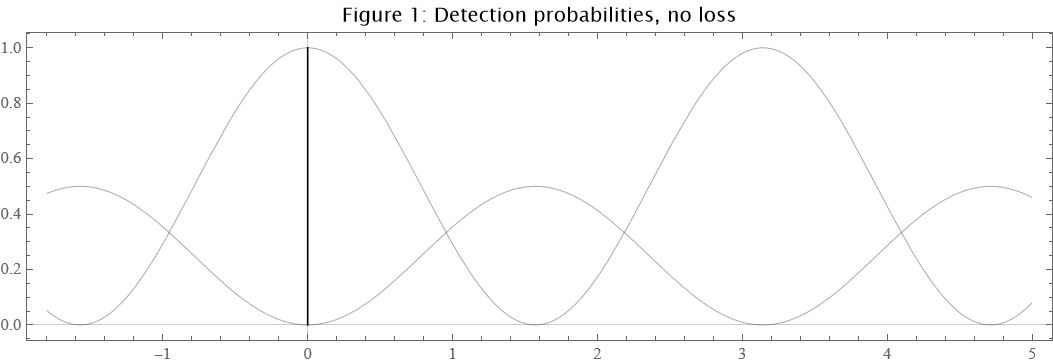
\includegraphics[width=0.9\textwidth]{figure/2024-08-25-16-28-48.png}
\label{fig:2024-08-25-16-28-48}
\end{figure}




\begin{figure}[htbp]
\centering
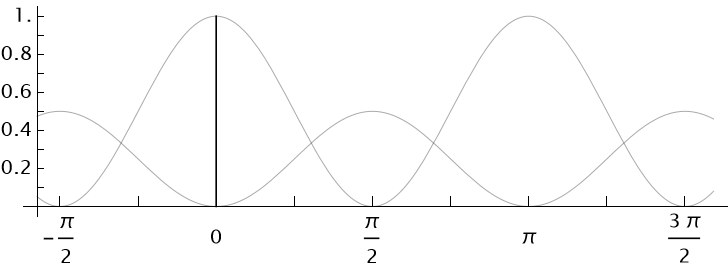
\includegraphics[width=0.9\textwidth]{figure/2024-08-25-17-11-08.png}
\label{fig:2024-08-25-17-11-08}
\end{figure}




\LaTeX{} is great at typesetting mathematics. Let $X_1, X_2, \ldots, X_n$ be a sequence of independent and identically distributed random variables with $\text{E}[X_i] = \mu$ and $\text{Var}[X_i] = \sigma^2 < \infty$, and let
\[S_n = \frac{X_1 + X_2 + \cdots + X_n}{n}
      = \frac{1}{n}\sum_{i}^{n} X_i\]
denote their mean. Then as $n$ approaches infinity, the random variables $\sqrt{n}(S_n - \mu)$ converge in distribution to a normal $\mathcal{N}(0, \sigma^2)$.


\subsection{How to change the margins and paper size}

Usually the template you're using will have 
the page margins and paper size set correctly for that use-case. For example, if you're using a journal article template provided by the journal publisher, that template will be formatted according to their requirements. In these cases, it's best not to alter the margins directly.

If however you're using a more general template, such as this one, and would like to alter the margins, a common way to do so is via the geometry package. You can find the geometry package loaded in the preamble at the top of this example file, and if you'd like to learn more about how to adjust the settings, please visit this help article on \href{https://www.overleaf.com/learn/latex/page_size_and_margins}{page size and margins}.

\subsection{How to change the document language and spell check settings}

Overleaf supports many different languages, including multiple different languages within one document. 

To configure the document language, simply edit the option provided to the babel package in the preamble at the top of this example project. To learn more about the different options, please visit this help article on \href{https://www.overleaf.com/learn/latex/International_language_support}{international language support}.

To change the spell check language, simply open the Overleaf menu at the top left of the editor window, scroll down to the spell check setting, and adjust accordingly.

\subsection{How to add Citations and a References List}

You can simply upload a \verb|.bib| file containing your BibTeX entries, created with a tool such as JabRef. You can then cite entries from it, like this: \cite{greenwade93}. Just remember to specify a bibliography style, as well as the filename of the \verb|.bib|. You can find a \href{https://www.overleaf.com/help/97-how-to-include-a-bibliography-using-bibtex}{video tutorial here} to learn more about BibTeX.

If you have an \href{https://www.overleaf.com/user/subscription/plans}{upgraded account}, you can also import your Mendeley or Zotero library directly as a \verb|.bib| file, via the upload menu in the file-tree.











\tikzset{every picture/.style={line width=0.75pt}} %set default line width to 0.75pt        


\begin{figure}[h]
\begin{center}
\begin{tikzpicture}[x=0.75pt,y=0.75pt,yscale=-1,xscale=1]
%uncomment if require: \path (0,1408); %set diagram left start at 0, and has height of 1408

%Straight Lines [id:da2745959879839548] 
\draw    (186.8,959) -- (270.8,959) ;

% Text Node
\draw    (373, 979.32) circle [x radius= 13.46, y radius= 13.46]   ;
\draw (368,970.82) node [anchor=north west][inner sep=0.75pt]   [align=left] {};
% Text Node
\draw    (251, 1015.82) circle [x radius= 13.04, y radius= 13.04]   ;
\draw (246,1007.82) node [anchor=north west][inner sep=0.75pt]   [align=left] {};
% Text Node
\draw    (372, 1064.82) circle [x radius= 13.04, y radius= 13.04]   ;
\draw (367,1056.82) node [anchor=north west][inner sep=0.75pt]   [align=left] {};
% Text Node
\draw (263.22,993.22) node [anchor=north west][inner sep=0.75pt]  [rotate=-341.24]  {$out$};
% Text Node
\draw (134,1008.8) node [anchor=north west][inner sep=0.75pt]    {$in$};
% Text Node
\draw (184,932.8) node [anchor=north west][inner sep=0.75pt]    {$system\ function$};
% Text Node
\draw (195.6,1069.4) node [anchor=north west][inner sep=0.75pt]   [align=left] {有向无环图};
% Connection
\draw    (263.89,1012.41) -- (358.2,983.81) ;
\draw [shift={(360.11,983.23)}, rotate = 163.13] [color={rgb, 255:red, 0; green, 0; blue, 0 }  ][line width=0.75]    (10.93,-3.29) .. controls (6.95,-1.4) and (3.31,-0.3) .. (0,0) .. controls (3.31,0.3) and (6.95,1.4) .. (10.93,3.29)   ;
% Connection
\draw    (263.48,1021.37) -- (357.66,1059.51) ;
\draw [shift={(359.52,1060.26)}, rotate = 202.05] [color={rgb, 255:red, 0; green, 0; blue, 0 }  ][line width=0.75]    (10.93,-3.29) .. controls (6.95,-1.4) and (3.31,-0.3) .. (0,0) .. controls (3.31,0.3) and (6.95,1.4) .. (10.93,3.29)   ;
% Connection
\draw    (153,1016.39) -- (235.54,1016.33) ;
\draw [shift={(237.54,1016.33)}, rotate = 179.96] [color={rgb, 255:red, 0; green, 0; blue, 0 }  ][line width=0.75]    (10.93,-3.29) .. controls (6.95,-1.4) and (3.31,-0.3) .. (0,0) .. controls (3.31,0.3) and (6.95,1.4) .. (10.93,3.29)   ;

\end{tikzpicture}
\caption{这是一个有向无环图的示例}
\label{fig:dag}
\end{center}
\end{figure}


如图 \ref{fig:dag} 所示,这是一个简单的有向无环图。








\vspace{1cm}

\tikzset{every picture/.style={line width=0.75pt}} %set default line width to 0.75pt        

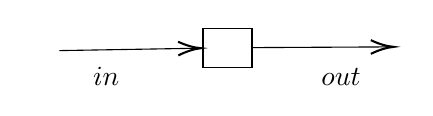
\begin{tikzpicture}[x=0.75pt,y=0.75pt,yscale=-1,xscale=1]
%uncomment if require: \path (0,300); %set diagram left start at 0, and has height of 300


% Text Node
\draw (282,148.4) node [anchor=north west][inner sep=0.75pt]    {$out$};
% Text Node
\draw    (226.19,130.07) -- (249.81,130.07) -- (249.81,148.93) -- (226.19,148.93) -- cycle  ;
\draw (245.37,133.83) node [anchor=north west][inner sep=0.75pt]  [rotate=-92.62]  {$$};
% Text Node
\draw (142,133.4) node [anchor=north west][inner sep=0.75pt]    {$$};
% Text Node
\draw (321,131.4) node [anchor=north west][inner sep=0.75pt]    {$$};
% Text Node
\draw (172,147.4) node [anchor=north west][inner sep=0.75pt]    {$in$};
% Connection
\draw    (157,140.85) -- (223.19,139.72) ;
\draw [shift={(225.19,139.69)}, rotate = 179.03] [color={rgb, 255:red, 0; green, 0; blue, 0 }  ][line width=0.75]    (10.93,-3.29) .. controls (6.95,-1.4) and (3.31,-0.3) .. (0,0) .. controls (3.31,0.3) and (6.95,1.4) .. (10.93,3.29)   ;
% Connection
\draw    (249.81,139.41) -- (316,139.06) ;
\draw [shift={(318,139.05)}, rotate = 179.69] [color={rgb, 255:red, 0; green, 0; blue, 0 }  ][line width=0.75]    (10.93,-3.29) .. controls (6.95,-1.4) and (3.31,-0.3) .. (0,0) .. controls (3.31,0.3) and (6.95,1.4) .. (10.93,3.29)   ;

\end{tikzpicture}




\subsection{Good luck!}

We hope you find Overleaf useful, and do take a look at our \href{https://www.overleaf.com/learn}{help library} for more tutorials and user guides! Please also let us know if you have any feedback using the Contact Us link at the bottom of the Overleaf menu --- or use the contact form at \url{https://www.overleaf.com/contact}.

\bibliographystyle{alpha}
\bibliography{sample}

\end{document}